\documentclass[a4paper,11pt]{article}
\usepackage[utf8]{inputenc}

% extra packages
% \usepackage{amsrefs}
% \usepackage[autocite=inline,labelalpha=true]{biblatex}

\usepackage[top=1in, left=1in, right=1in, bottom=1in]{geometry}
\usepackage{geometry}
\usepackage{amsmath, amssymb}
\usepackage{graphicx}
\usepackage{color}
\usepackage{hyperref}
\usepackage{siunitx}

\newcommand{\ve}{\varepsilon}
\newcommand{\h}{\mathcal{H}}

%\setlength{\parindent}{0pt}

\begin{document}

\begin{center}
\Large \textbf{Research Statement}

\Large Youngmin Park
\end{center}

\section{Introduction}

I develop dimension-reduction methods for neural network models using stochastic and deterministic \textbf{dynamical systems theory}, and in turn, use these findings to understand how biological neural networks function and how they are maintained. I also specialize in \textbf{interdisciplinary research with excellent funding potential}. My publication record demonstrates my ability to produce high-impact work with researchers of diverse backgrounds including neuroscientists \cite{park2020circuit}, engineers \cite{ermentrout2019recent,park2020high}, mathematical neuroscientists \cite{park2016weakly,park2018infinitesimal,park2018multiple,park2018scalar}, and fluid dynamicists \cite{park2020dynamics}. My research program includes the following sub-directions:

\begin{itemize}
	\item \textbf{Coupled oscillators, Section \ref{sec:interactions}}. In summary, I introduce a generalization of weakly coupled oscillator theory to strong coupling. This work will allow mathematician to include subtle but important details in reduced phase models that are often neglected by idealized models. This work opens the way for a thorough re-examination of decades of existing oscillator theory using realistic models as opposed to highly constrained or unrealistic models. There is excellent potential to sharpen general questions regarding network dynamics in physics, chemistry, and biology.
	\item \textbf{Molecular motors, Section \ref{sec:maintenance}}. In summary, I analyze a model of molecular transport, where vesicles are forced into nanometer-scale cell compartments. My work suggests that fluid dynamics forces, molecular motor forces, and the shape of the confinement play significant factors in neural maintenance. This work opens the way for detailed, tractable studies on neural maintenance and how defects in maintenance affect brain function. The long-term goal of this work is to help understand the causes and mechanisms behind brain disorders such as Alzheimer's.
	\item \textbf{Cortical network analysis and machine learning, Section \ref{sec:data}}. In summary, I introduced an idealized model of the auditory cortex, which unified disparate optogenetics results in the literature. The model serves as a proof of concept that large numbers of computations in the brain may be handled efficiently by relatively simple neural circuits. This work is an excellent starting point to gain a deeper understanding into the principles underlying general sensory processing. The goal is to create biologically-inspired artificial neural networks which may learn more quickly and robustly than existing methods.
	\item \textbf{Undergraduate research, Section \ref{sec:undergrad}}. In summary, my work is accessible to a broad spectrum of skills and backgrounds in STEM (although I strongly encourage students from other backgrounds to participate in my research). My goal is to equip students with skills such as programming and scientific literacy, which they can use to enhance their lives and careers.
\end{itemize}
%I conclude with a comprehensive research plan in Section \ref{sec:research}.

\section{Coupled Oscillators}\label{sec:interactions}

My work on oscillations falls within the broader work of oscillator theories oriented towards understanding pathological neural behavior such as Parkinsonian tremors, epilepsy, and cardiac alternans. The weak coupling assumption has long been an invaluable theoretical tool to understand neural behavior consisting of only small deviations from a known behavior such as quiescence or oscillatory activity \cite{ermentrout2002modeling,park2016weakly,park2018multiple,park2018scalar}. However, modern experiments are often done \textit{in vivo}, where neurons are often strongly coupled, heterogeneous, and interact nonlinearly. These properties hold in both normal and pathological neural function, so it follows that pathologies can not always be understood using abstraction, symmetry, or linearity. Therefore, my field must develop theories that directly address \textit{strongly coupled} networks of \textit{heterogeneous} neurons with \textit{nonlinear} interactions at multiple scales. We must understand the brain as it is.

To this end, \textit{I have formulated a theory of strongly coupled oscillators} \cite{park2020high}. I tested this theory using a realistic four-dimensional model of a thalamic neuron. Figure \ref{fig:thal} shows how my theory predicts phase differences in two thalamic oscillators for different coupling strengths (higher order corresponds to greater accuracy). The right-hand side of the reduced ODE (labeled $-2\h_{\text{odd}}$) is shown in the top row. Roots and slopes correspond to existence and stability of phase-locked states. Phase differences of the full model is shown in the bottom row for 20 difference initial conditions. Coupling strength increases from weak ($g_\text{syn}=0.02$, left column) to strong ($g_\text{syn}=0.25$, right column). \textit{Roots of the fourth-order reduction coincide with the steady-state phase-locked states of the full system}.

\begin{figure}[ht!]
	\centering
	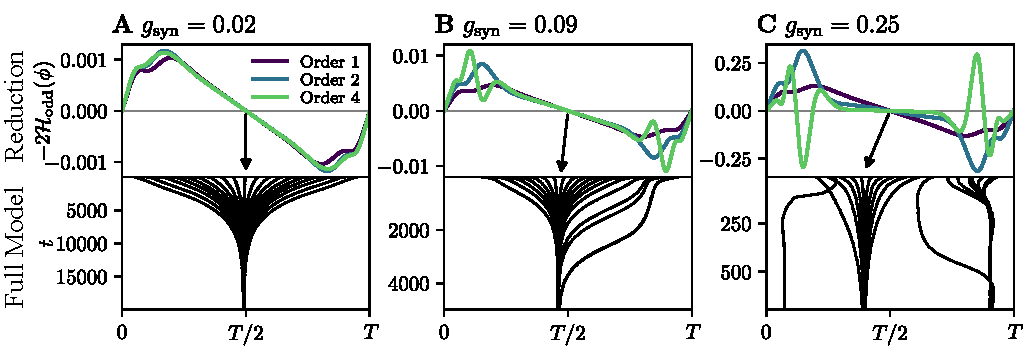
\includegraphics[width=\textwidth]{figures/thal_h_edited.pdf}
	\caption{Performance of the strong coupling reduction compared to a full simulation of thalamic neuron models. A: Weak coupling. The right-hand side of the reduction (top) is shown for different orders (higher is more accurate) and coincides with the long-term phase difference of the full model (bottom). B: Moderate coupling. The reduction (top) coincides with the full model (bottom). C: Strong coupling. The reduction (top) only agrees with the full model (bottom) at order 4. }\label{fig:thal}
\end{figure}

In the long term, I will further develop mathematical methods to analyze neural networks in several important directions. I will augment my theory to include heterogeneity (including n:m phase-locking), making my theory applicable to far more realistic neural networks. I will augment my theory to include oscillator death to understand interactions between bursting neurons in networks such as subcortical networks and central pattern generators. Finally, I will derive the mean-field equations for neural models (in contrast to existing mean-field theories that use idealized models \cite{ott2008low}) to understand how microscopic neural interactions influence large-scale brain activity.

\section{Neural Maintenance: Dendritic Spines} \label{sec:maintenance}

Pyramidal neurons, the most ubiquitous type of neurons in the mammalian neocortex. They feature tens of thousands of excitatory convergent synaptic inputs, where most incoming synaptic signals terminate on sub-micron bulbs known as dendritic spines \cite{nimchinsky2002structure}. Spines exhibit a significant degree of morphological plasticity, with pathological spine formation implicated in disorders such as Autism spectrum disorder and Alzheimer's disease. How spines function and how they are maintained is therefore an important question.

%\cite{park2006plasticity,wang2008myosin}
Dendritic spines receive surface proteins by protein-carrying vesicles that squeeze through the neck of the spine and eventually fuse with the spine head. The motion of such vesicles has been observed to not involve only translocation, where the motion is unidirectional, but includes corking, where the vesicle gets ``stuck'' in the spine neck, and rejection, where the vesicle initially enters the spine but eventually reverses direction and exits. \textit{How molecular motors affect changes in vesicle direction is the goal of ongoing work} \cite{park2020dynamics}.

While mean-field models are useful with large numbers of agents, sub-micron spines only contain a few dozen myosin motors. \textit{The effects of noise are prominent, and we can not rely on mean-field models to fully understand how spines function}. Thus I will shift my attention to understanding how finite numbers of stochastic motors affect the probability of translocation.


\section{Cortical Network Analysis and Machine Learning}\label{sec:data}

I introduced an idealized model of the auditory cortex unifying numerous experimental results in the field of auditory neuroscience \cite{park2020circuit}. This model demonstrated that simple cortical mechanisms including synaptic facilitation and depression are sufficient to reproduce numerous types of auditory processing. The model included excitatory (pyramidal) neurons as well as the inhibitory subtypes somatostatin-positive (SOM) and parvalbumin-positive (PV) interneurons, which were necessary to reproduce optogenetic results. While we performed some parameter sweeps, the ability of the model to reproduce additional auditory phenomena was not explored in depth. Many questions remain regarding robustness of the model and its similarity to real cortical networks. In addition, questions remain regarding how this model can be used to constrain artificial neural networks to reduce learning iterations. This problem is general and aligns with machine learning researchers in other fields who are seeking to add physical constraints neural networks in fluid dynamics \cite{mohan2020embedding} and Earth science \cite{pelissier2020combining}.


%In addition, I worked with a neuroscientist at the Geffen lab who ran auditory experiments on mice. They generated many gigabytes of partially-observed calcium traces, which were generated as the mouse responded to auditory tasks. In order to generate correlations between all observed neurons, I used subspace identification to recover correlations when pairs of neurons were not observed on a given trial. The method included the use of stochastic gradient descent to estimate the optimal correlation matrix corresponding to the partial data. Once this was performed, I used hierarchical clustering and found that correlated neurons tended to be spatially clustered in the cortex (unpublished).

%Machine learning is an incredibly powerful, general tool, yet learning algorithms then to be extremely expensive in terms of trials, requiring countless iterations. In contrast, animals tend to learn with far fewer iterations. I hypothesize that there exist neural networks with biologically-inspired constraints that are capable of learning far more rapidly than a general neural network. 



\section{Undergraduate Research}\label{sec:undergrad}

%Studying dynamical systems through the lens of biology is the perfect framework to involve a diverse group of undergraduates in research. Problems in mathematical biology are accessible to students from several STEM fields with just a basic understanding of calculus and ordinary differential equations. Such students can bring their own knowledge of math, biology, ecology, chemistry, physics, or computer science and learn fundamental mathematical modeling techniques along the way. The principles they will learn from formalizing a problem within a mathematical framework will teach them to extract essential characteristics of a system in order to generalize other properties. This method of thinking will serve them well throughout their undergraduate education and further into their careers.

Virtually any STEM student with a basic understanding of calculus and ordinary differential equations will be able to contribute to my research. My students will first learn the fundamentals of the field of their choosing. Driven students will have the opportunity to publish first- and second-author papers in reputable journals. My goal is to provide undergraduates many opportunities to learn important and relevant skills. They will learn to communicate in speech and writing by interacting with others of different backgrounds.

Below are potential project ideas from simple to complex, to be given depending on the skill, interest, and commitment time of the student. I remark that I fully understand the potential for a relatively unskilled and uninterested student to turn into a skilled and dedicated researcher, so this list is by no means a hard rule.

\begin{itemize}
	\item (Simple) Reproduce figures from a paper of the student's choosing and present on the main results. Generate potential research ideas based on the paper.
	\item (Simple) Help improve the documentation for my open source projects in coupled oscillators and molecular motor dynamics. Contribute features to these projects.
	\item (Moderate) Join an ongoing research project. For example, generate figures for a paper using a language and numerical integrator of their choosing. The student will be tasked with visualizing a particular problem and will be responsible for writing and debugging their own code from top to bottom.
	\item (Complex) Lead a research project. For example, study the effects of splay states using strong oscillator coupling theory. Determine different types of bifurcations as a network transitions from different phase-locked states as a function of a network parameter, such as coupling strength.
\end{itemize}

%The Fokker-Planck equation and corresponding Langevin equation would have been ideal, but they fail to work for our system, which is a class of birth-death models \cite{doering2005extinction}. I have therefore turned to the master equation, which presents its own set of challenges. In existing literature, molecular motors typically do not have spatial dynamics, and have position-independent attachment and detachment rates. A master equation formulation is therefore very straightforward to derive. In contrast, the myosin motor depends on position and velocity, which affect the detachment rates in a way that standard steady-state assumptions are not valid. To account for the dependencies, I included the appropriate position and velocity dependencies into a modified version of the master equation. Some problems remain to be ironed out, but this master equation largely reproduces the MFPT of the agent-based model with a speed improvement in two orders of magnitude.

%I will turn to the question of how constrictions affect the probability of vesicle translocation and compute the mean first passage time of vesicle translocation. Due to the increasing complexity of the model, I may turn to additional simplifying assumptions and further abstract the model to make this question tractable. The future directions beyond this point are plentiful. For example, protein-carrying vesicles serve as part of a greater maintenance complex that includes maintaining the receptor density, modifying the spine shape and size, and increasing the reliability of postsynaptic spine responses. I will pursue questions on how translocation affects the function of the greater complex, and how the spine maintains an optimal shape for a given function.

%\section{Research Plan}\label{sec:research}

%The long-term goal of my research is twofold. First, to further develop new dimension reduction strategies that can be used to understand neural interactions and neural maintenance, and second, to combine the research insights from my work to build a comprehensive understanding of brain function. In my future research, I will research how the maintenance of individual spines affect the neural response properties of synapses distributed throughout neurons and networks. This work naturally relates to understanding how changes in dendritic spines affect the communication of neurons in brain networks, and leads to a holistic understanding of how neural dysfunction affect disorders such as Alzheimer's and autism.

%My overall research is mathematical, computational, and biological. It provides ample opportunities for students at any level to engage in state-of-the-art multidisciplinary research. Preferred backgrounds include (but are not limited to ) mathematics, biology, computer science, physics, and chemistry. Because my work is at the intersection of many fields, my students will learn to communicate with people of diverse backgrounds, and will learn general methods in mathematics and programming.


\bibliographystyle{plain}
\bibliography{refs.bib,../youngmin-bard/bio,../youngmin-bard/neuralfield,../youngmin-bard/math,../youngmin-bard/phase,../youngmin-bard/computation,../youngmin-bard/cortex,../thomas-youngmin/notes/spines.bib,../thomas-youngmin/notes/vesicles.bib,../thomas-youngmin/notes/noise.bib,../thomas-youngmin/notes/motors.bib}


\end{document}
